\chapter{آزمایش و نتایج}
\section{ساختار نرم‌افزاری \lr{Kompute}}
به منظور تست الگوریتمی که در بخش پیشین ارائه گردید، یک ساختار نرم‌افزاری (فریم‌ورک) با نام \lr{Kompute} در زبان \lr{Kotlin} تعبیه شده است که مخزن آن در لینک زیر در دسترس می‌باشد:
\begin{latin}
	\begin{itemize}
		\item \href{https://github.com/dalisyron/Kompute}{https://github.com/dalisyron/Kompute}
	\end{itemize}
\end{latin}
با استفاده از این فریم‌ورک می‌توان الگوریتم جستجوی استراتژی تخلیه بهینه را به ازای پارامترهای محیطی مختلف اجرا کرد و عملکرد استراتژی بدست آمده از الگوریتم را با کمک شبیه‌سازی با سایر استراتژی‌ها مقایسه کرد. این فریم‌ورک طبق یافته‌های ما اولین پیاده‌سازی متن‌باز در زمینه استراتژی تخلیه وظایف ناهمگون است. \\

معماری کلی این فریم‌ورک در قالب یک کلاس دیاگرام در صفحه بعد آورده شده است.
\newpage
\begin{figure}[H]
	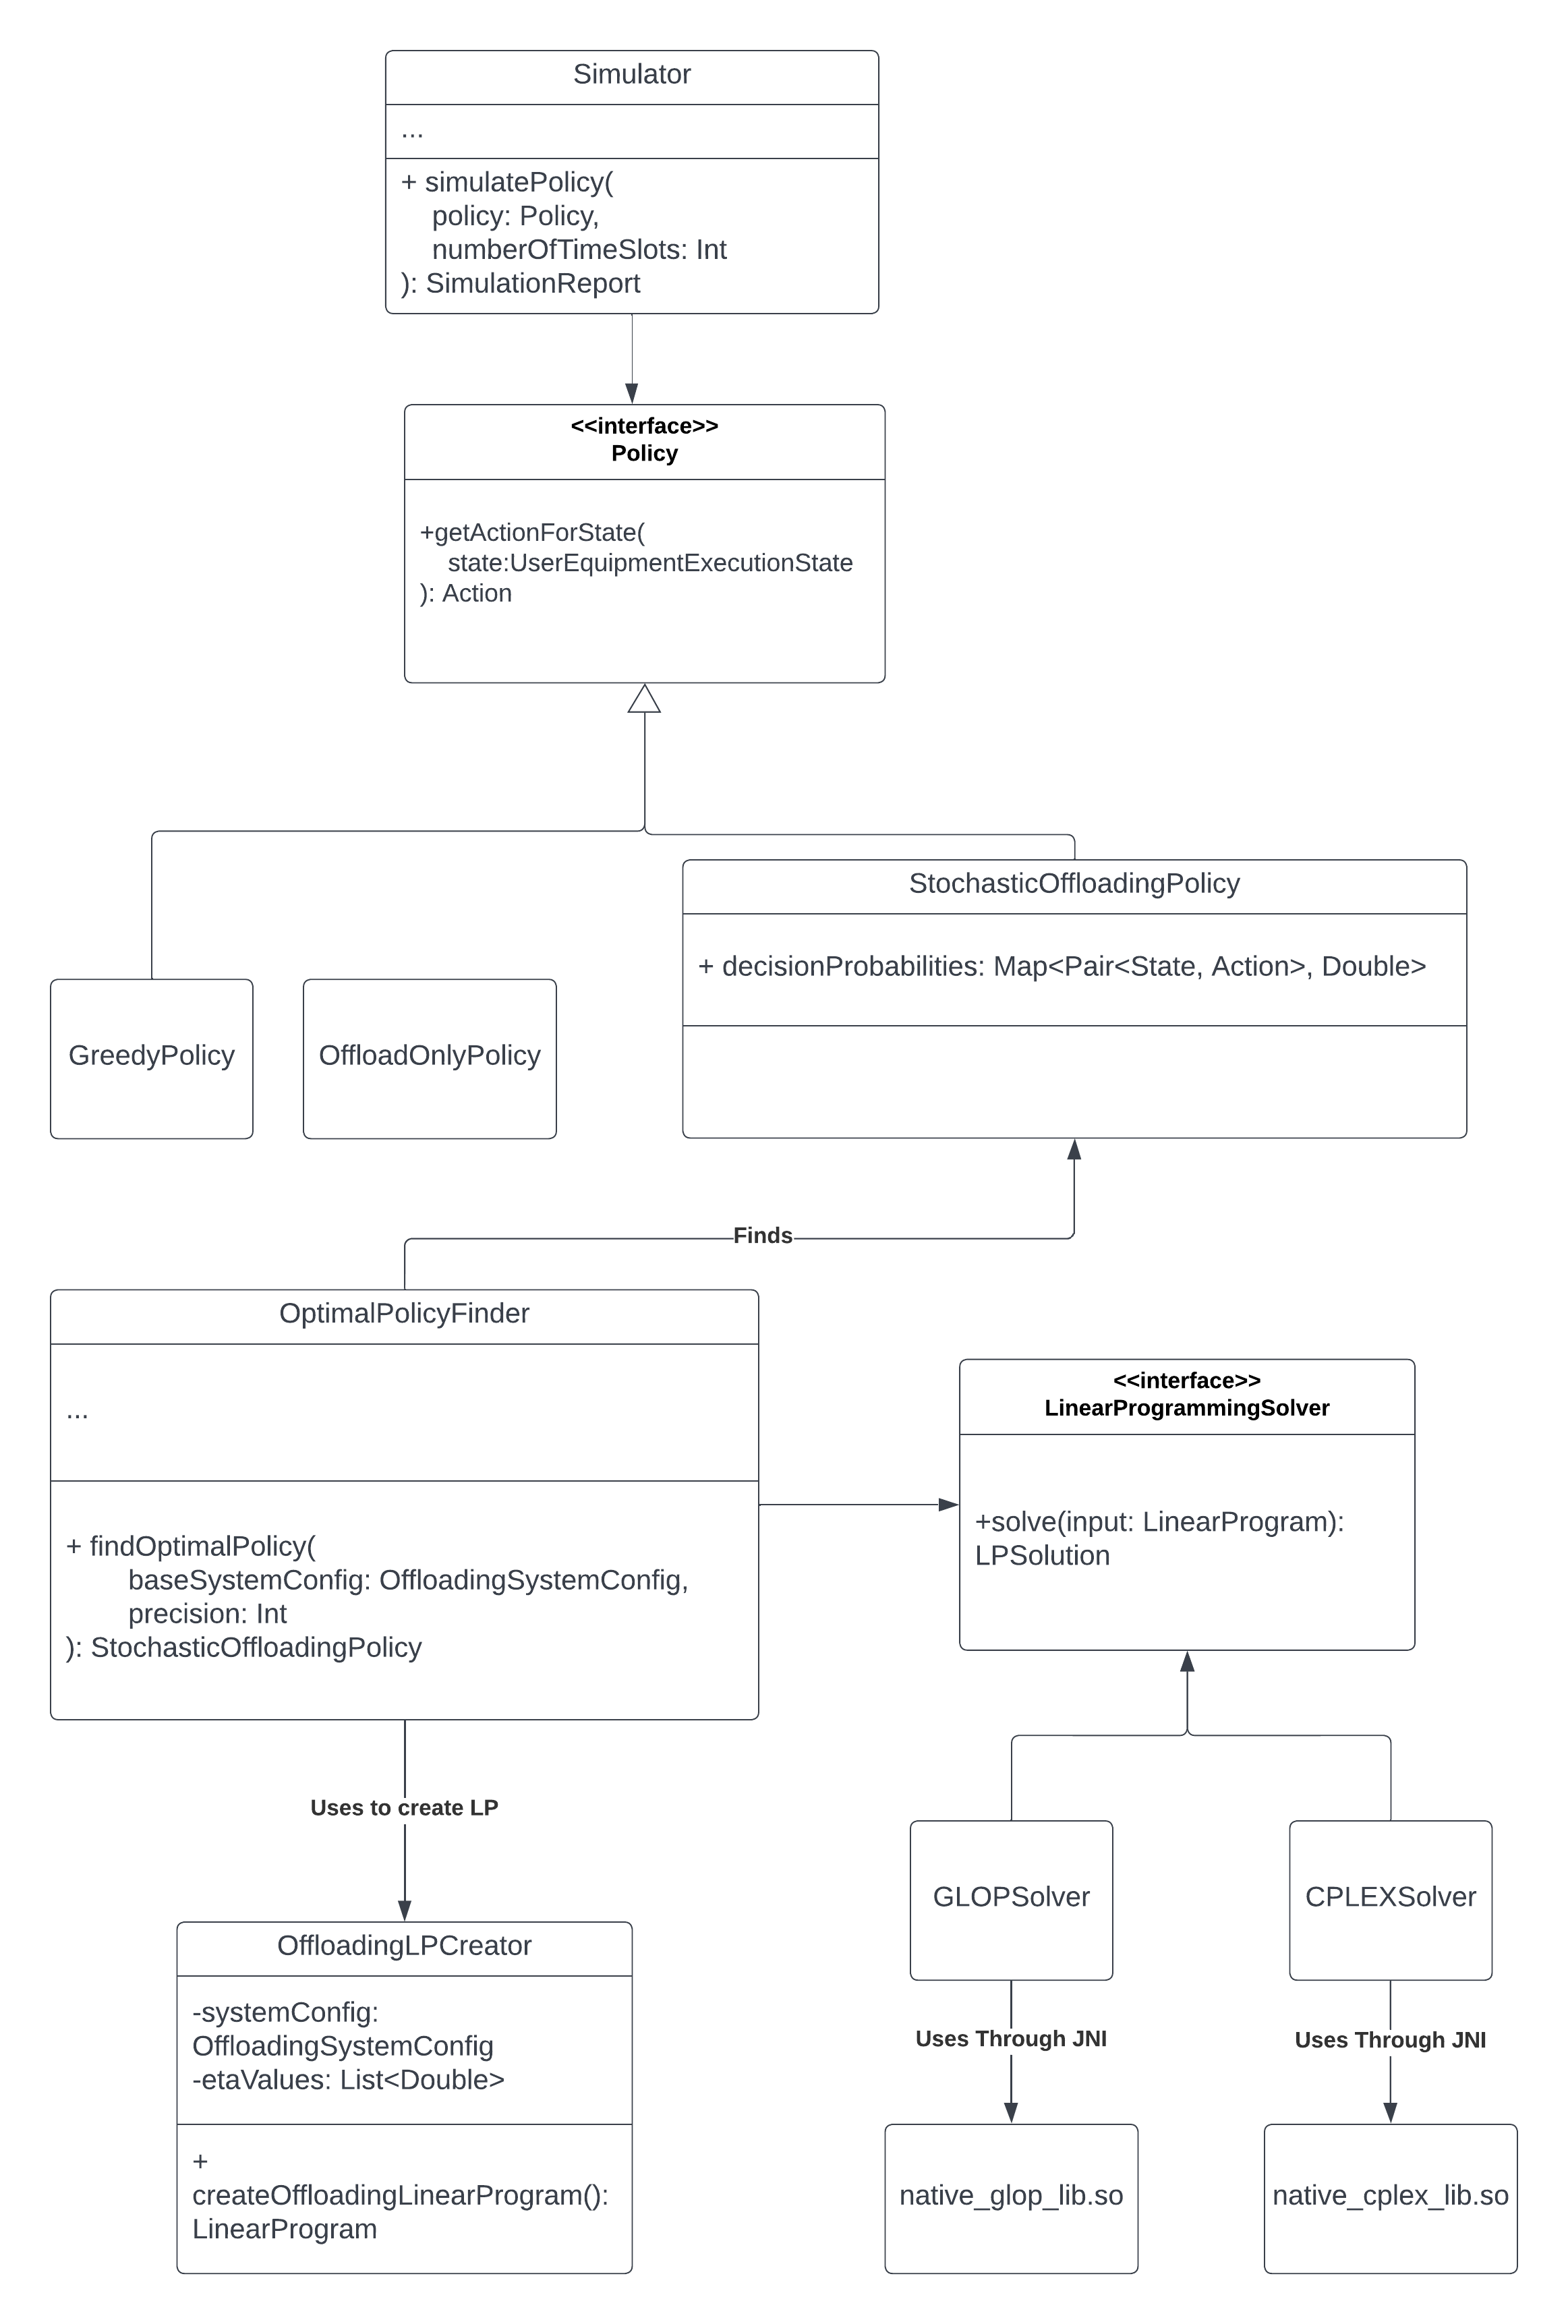
\includegraphics[width=0.9\textwidth]{cdiagram.png}
	\caption{کلاس دیاگرام فریم‌ورک \lr{Kompute}}
\end{figure}
\newpage
\subsection{ساخت و حل یک مسئله تخلیه وظیفه نمونه در \lr{Kompute}}
در کد نمونه زیر مسئله تخلیه وظیفه‌ برای محیط رایانش لبه‌ای با دو صف\footnote{شرایط بر اساس تقسیم‌بندی وظایف به \lr{Heavy} و \lr{Light} در اینترنت اشیا} حل شده است.
\begin{latin}
\begin{lstlisting}[language=Kotlin]
fun main(args: Array<String>) {
	val systemConfig = OffloadingSystemConfig(
		userEquipmentConfig = UserEquipmentConfig(
			stateConfig = UserEquipmentStateConfig(
				taskQueueCapacity = 5,
				tuNumberOfPackets = listOf(1, 3),
				cpuNumberOfSections = listOf(7, 2),
				numberOfQueues = 2
			),
			componentsConfig = UserEquipmentComponentsConfig(
				alpha = listOf(0.4, 0.9),
				beta = 0.90,
				etaConfig = null,
				pTx = 1.0,
				pLocal = 0.8,
				pMax = 1.7
			)
		),
		environmentParameters = EnvironmentParameters(
			nCloud = listOf(1, 1),
			tRx = 0.5,
		)
	)
	
	val optimalPolicy = RangedOptimalPolicyFinder.findOptimalPolicy(
		baseSystemConfig = systemConfig, 
		precision = 10
	)
	/*
	// For multi-threaded execution use this instead:
	
	val optimalPolicy = ConcurrentRangedOptimalPolicyFinder(
		baseSystemConfig = systemConfig
	).findOptimalPolicy(precision = 10, numberOfThreads = 8)
	*/
	
	
	val decisionProbabilities: Map<StateAction, Double>
	= optimalPolicy.stochasticPolicyConfig.decisionProbabilities
	
	println(decisionProbabilities)
}
\end{lstlisting}
\end{latin}
\newpage
\section{نتایج شبیه‌سازی}
در این بخش عملکرد استراتژی یافت شده توسط الگوریتم \ref{alg:cap} را با چهار الگوریتم پایه زیر مقایسه می‌کنیم:
\begin{enumerate}
	\item استراتژی «فقط تخلیه»\LTRfootnote{Offload Only} که همه‌ی وظایف را تخلیه می‌کند
	\item استراتژی «حریصانه، تخلیه اول»\LTRfootnote{Greedy (Offload First)} که در هر بازه زمانی اگر واحد ارسال یا پردازنده بیکار باشند به هر کدام از آنها یک وظیفه از صفی رندوم تخصیص می‌دهد و در صورتی که تنها یک وظیفه در صف باشد و مجبور به انتخاب بین تخلیه و اجرای محلی باشد، تخلیه را انتخاب می‌کند.
	\item استراتژی «حریصانه، محلی اول»\LTRfootnote{Greedy (Local First)} که در هر بازه زمانی اگر واحد ارسال یا پردازنده بیکار باشند به هر کدام از آنها یک وظیفه از صفی رندوم تخصیص می‌دهد و در صورتی که تنها یک وظیفه در صف باشد و مجبور به انتخاب بین تخلیه و اجرای محلی باشد، اجرای محلی را انتخاب می‌کند.
	\item استراتژی «فقط (اجرای) محلی»\LTRfootnote{Local Only}
\end{enumerate}
\newpage
\subsection{شبیه‌سازی تک صف}
با توجه به اینکه روش ارائه شده توسط ما حالت گسترش یافته \cite{Liu} است، ابتدا محیط تست ارائه شده در آن پژوهش را برای تست الگوریتم در نظر می‌گیریم. پارامترهای این محیط در جدول \ref{table:parameters-singlequeue} خلاصه شده اند. نتیجه این آزمایش در شکل \ref{plot:singleQueue} مشاهده می‌شود.

% Please add the following required packages to your document preamble:
\begin{table}[H]
	\centering
	\begin{latin}
		\begin{tabular}{@{}lllllllll@{}}
			\toprule
			\textbf{Parameter} & $M_1$ & $L_1$ & $\beta$ & $P_{tx}$ & $P_{loc}$ & $P_{max}$ & $C_1$ & $t_{rx}$ \\ \midrule
			\textbf{Value}             & 1    & 17   & 0.4  & 1.0 & 0.8  & 1.6  & 1    & 0.0   \\ \bottomrule
		\end{tabular}
	\end{latin}
	\caption{پارامترهای محیط رایانش لبه‌ای در سناریو تک صف}
	\label{table:parameters-singlequeue}
\end{table}

\begin{figure}[H]
	\centering
	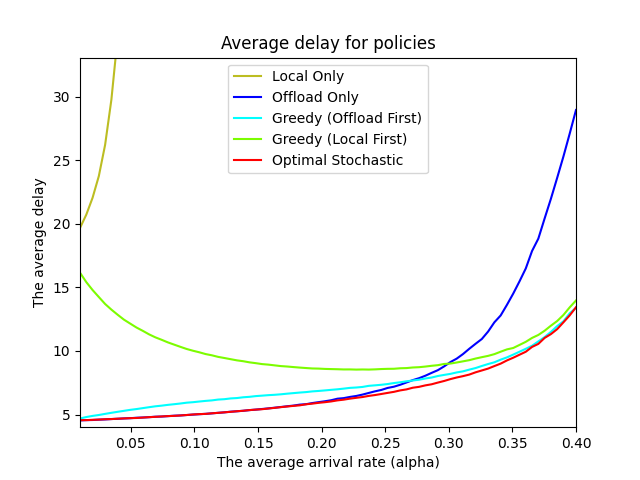
\includegraphics[width=0.7\textwidth]{PlotLiuLimitedSingleQueue.png}
	\caption{تاخیر سرویس به ازای نرخ ورود در حالت تک صف}
	\label{plot:singleQueue}
\end{figure}
همانطور که مشاهده می‌شود استراتژی تخلیه تصادفی یافت شده از تمام الگوریتم‌های پایه بهتر عمل می‌کند و شکل منحنی‌های نمودار با \cite{Liu} مطابقت دارد.
\newpage
\subsubsection{شبیه‌سازی دو صف با یک صف ثابت در سناریو سبک و سنگین}
در این قسمت سناریوی تست به این گونه است که میزان تاخیر به ازای مقادیر مختلف نرخ ورود برای صف شماره یک و مقدار ثابت نرخ ورود برای صف شماره دو مشاهده می‌شود. پارامترهای محیطی در نظر گرفته شده در جدول \ref{table:fixedranged} به طور خلاصه آمده است.
\begin{figure}[H]
	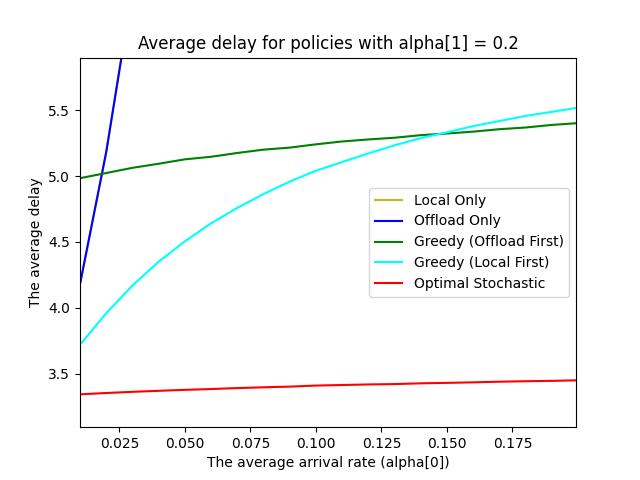
\includegraphics[width=\textwidth]{FixedRanged.png}
\end{figure}
% Please add the following required packages to your document preamble:
% \usepackage{booktabs}
\begin{table}[H]
	\centering
	\begin{latin}
		\begin{tabular}{@{}llllllllllll@{}}
			\toprule
			\textbf{Parameter} & $M_1$ & $M_2$ & $L_1$ & $L_2$ & $C_1$ & $C_2$ & $\beta$ & $P_{tx}$ & $P_{loc}$ & $P_{max}$ & $t_{rx}$ \\ \midrule
			\textbf{Value}     & 1     & 3     & 7     & 2     & 1     & 1     & 0.95    & 1        & 0.8       & 1.6       & 0        \\ \bottomrule
		\end{tabular}
	\end{latin}
	\caption{پارامترهای محیط رایانش لبه‌ای در سناریو دو صف با یک صف ثابت}
	\label{table:fixedranged}
\end{table}
همانطور که مشاهده می‌شود استراتژی تخلیه بهینه بسیار بهتر از الگوریتم‌های پایه عمل می‌کند. دلیل اصلی این تفاوت زیاد (نسبت به تفاوت کم در سناریو با یک صف در بخش قبل) عدم هوشمندی استراتژی‌های حریصانه در انتخاب نوع وظیفه تخصیص داده شده به پردازنده و واحد ارسال است. به عبارت دیگر انتخاب تصادفی نوع وظیفه فرستاده شده به پردازنده و واحد ارسال در الگوریتم‌های حریصانه باعث می‌شود که در شرایطی که تفاوت زیادی بین نوع وظایف وجود دارد (مانند سناریو سبک و سنگین) این الگوریتم‌ها عملکرد خیلی بدی داشته باشند. این در حالی است که در حالت تک صف انتخاب بین انواع وظیفه مطرح نبوده است و تنها عامل برای عملکرد غیربهینه‌ی استراتژی‌های حریصانه، عدم زمانبندی درست وظایف بوده است.
\newpage
\subsubsection{شبیه‌سازی دو صف متغیر وظایف سبک و سنگین}
\label{sub:heavylight}
در این قسمت مقدار تاخیر سرویس به ازای مقادیر مختلف نرخ ورود به هر دو صف محاسبه شده است. پارامترهای سیستمی این سناریو در جدول \ref{table:double} آمده است. همانطور که مشاهده می‌شود استراتژی بهینه در بازه 
$\alpha_1, \alpha_2 \in [0, 0.4]$
عملکرد قابل قبول دارد.
\begin{figure}[H]
	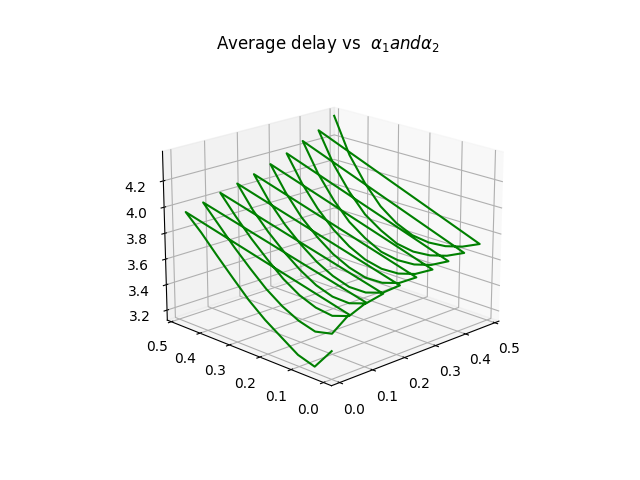
\includegraphics[width=\textwidth]{Plot3d.png}
\end{figure}
\begin{table}[H]
	\centering
	\begin{latin}
		\begin{tabular}{@{}llllllllllll@{}}
			\toprule
			\textbf{Parameter} & $M_1$ & $M_2$ & $L_1$ & $L_2$ & $C_1$ & $C_2$ & $\beta$ & $P_{tx}$ & $P_{loc}$ & $P_{max}$ & $t_{rx}$ \\ \midrule
			\textbf{Value}     & 1     & 3     & 7     & 2     & 1     & 1     & 0.95    & 1        & 0.8       & 1.6       & 0        \\ \bottomrule
		\end{tabular}
	\end{latin}
	\caption{پارامترهای محیط رایانش لبه‌ای در سناریو دو صف متغیر}
	\label{table:double}
\end{table}
\newpage
\subsubsection{شبیه‌سازی سه صف وظیفه}
در این قسمت عملکرد الگوریتم ارائه شده در شرایطی که سه صف وجود دارد بررسی شده است. پارامترهای محیط رایانش لبه‌ای در جدول \ref{table:triple} آورده شده است. با توجه به اینکه رسم نمودار در شرایط چهار بعدی امکان پذیر نیست از مفهومی به نام آزمون «کارآمدی» استفاده می‌کنیم. مفهوم کارآمدی را اینگونه تعریف می‌کنیم که یک استراتژی کارآمد است اگر احتمال پر بودن یک یا چند صف در سیستم از 
$\frac{1}{|S|}$
کمتر باشد. در این آزمایش، کارآمدی استراتژی‌های مختلف را به ازای ۱۰۰۰ نمونه مختلف در بازه‌های 
$\alpha_1, \alpha_2, \alpha_3 \in [0, 0.2]$
 تست کردیم که نتایج آن در جدول \ref{table:triplequeuepercents} مشاهده می‌شود.
 
\begin{table}[H]
	\centering
	\begin{latin}		
		\resizebox{\textwidth}{!}{
		\begin{tabular}{llllll}
			\hline
			\textbf{Policy} & Optimal & Local Only & Greedy (Local First) & Greedy (Offload First) & Offload Only \\ \hline
			\textbf{Effectiveness}           & 100.0\%   & 8.5\%      & 80.3\%                & 79.3\%                  & 21.6\%        \\ \hline
		\end{tabular}
	}
	\end{latin}
	\caption{ درصد کارآمدی استراتژی‌ها}
	\label{table:triplequeuepercents}
\end{table}

% Please add the following required packages to your document preamble:
% \usepackage{booktabs}
\begin{table}[H]
	\centering
	\resizebox{\textwidth}{!}{
	\begin{latin}		
		\begin{tabular}{@{}lllllllllllllll@{}}
			\toprule
			Parameter & $M_1$ & $M_2$ & $M_3$ & $L_1$ & $L_2$ & $L_3$ & $C_1$ & $C_2$ & $C_3$ & $\beta$ & $P_{tx}$ & $P_{loc}$ & $P_{max}$ & $t_{rx}$ \\ \midrule
			Value     & 1     & 3     & 2     & 4     & 2     & 3     & 1     & 1     & 2     & 0.95    & 1        & 0.8       & 1.6       & 0.5      \\ \bottomrule
		\end{tabular}
	\end{latin}
		}
	\caption{پارامترهای محیط رایانش لبه‌ای در سناریو سه صف}
	\label{table:triple}
\end{table}
\clearpage
